\documentclass[tikz,border=3mm]{standalone}
\usepackage[T1]{fontenc}
\usepackage{lmodern}
\usetikzlibrary{arrows.meta,calc}
\definecolor{concrete}{HTML}{EAF3FB}
\definecolor{abstract}{HTML}{FFF3C4}
\definecolor{ink}{HTML}{444444}
\begin{document}
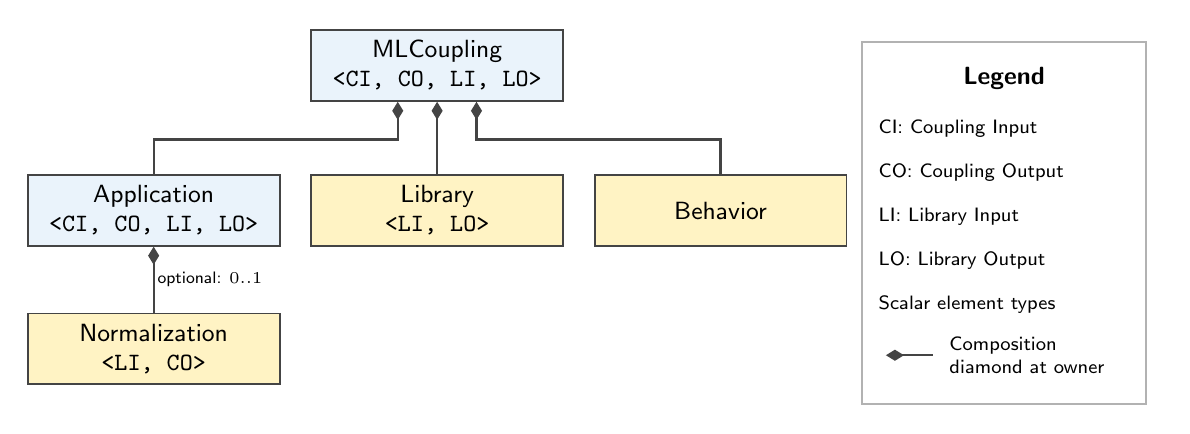
\begin{tikzpicture}[
  x=1mm,y=.8mm,font=\sffamily\fontsize{9}{10.5}\selectfont,
  class/.style={draw=ink,line width=.65pt,fill=concrete,
    minimum width=32mm,minimum height=9mm,align=center,inner sep=2pt},
  abstract/.style={class,fill=abstract},
  owns/.style={draw=ink,line width=.8pt,{Diamond[length=6.5pt,width=4pt]}-},
  label/.style={font=\sffamily\fontsize{6}{7}\selectfont,inner sep=1pt},
  note/.style={anchor=west,font=\sffamily\fontsize{7}{8.5}\selectfont,inner sep=0pt}
]
\path[use as bounding box] (0,-10) rectangle (144,-70);
\node[class] (coupling) at (52,-16) {MLCoupling\\\texttt{<CI, CO, LI, LO>}};
\node[class] (app) at (16,-39) {Application\\\texttt{<CI, CO, LI, LO>}};
\node[abstract] (lib) at (52,-39) {Library\\\texttt{<LI, LO>}};
\node[abstract] (beh) at (88,-39) {Behavior};
\draw[owns] ($(coupling.south)+(-5,0)$) -- ++(0,-6) -| (app.north);
\draw[owns] (coupling.south) -- (lib.north);
\draw[owns] ($(coupling.south)+(5,0)$) -- ++(0,-6) -| (beh.north);
\node[abstract] (norm) at (16,-61) {Normalization\\\texttt{<LI, CO>}};
\draw[owns] (app.south) -- node[label,right] {optional: $0..1$} (norm.north);

\node[class,fill=white,draw=gray!60,minimum width=36mm,minimum height=46mm]
  at (124,-41) {};
\node[font=\sffamily\fontsize{9}{10.5}\selectfont\bfseries] at (124,-18) {Legend};
\node[note] at (108,-26) {CI: Coupling Input};
\node[note] at (108,-33) {CO: Coupling Output};
\node[note] at (108,-40) {LI: Library Input};
\node[note] at (108,-47) {LO: Library Output};
\node[note] at (108,-54) {Scalar element types};
\draw[owns] (109,-62) -- (115,-62);
\node[note,align=left] at (117,-62) {Composition\\diamond at owner};
\end{tikzpicture}
\end{document}
